%\documentclass[compress,notesonly]{beamer} %compress to make bars as small as possible
                                           %notesonly to add note not visible on screen (\note[]{})
\documentclass[compress,slidescentered,notes=show]{beamer}
%\documentclass[compress,slidescentered,notes=hide]{beamer}

%---------------FONT AND LANGUAGES ---------------------------
\usepackage[utf8]{inputenc}
%\usepackage[T1]{fontenc}
\usepackage[english]{babel}
\usepackage{pifont}

%--------------FORM ------------------------------
%\usepackage{beamerthemesplit}
\usepackage{multicol} %possibility to create columns
\usepackage{comment} 
%\usepackage[absolute,showboxes, overlay]{textpos}
%\textblockorigin{1mm}{1mm}
%\TPshowboxestrue % or false to display contour
\usepackage{array}
\pdfpageattr {/Group << /S /Transparency /I true /CS /DeviceRGB>>}
\usenavigationsymbolstemplate{}

\usetheme{Darmstadt} %Frankfurt} 
%\useoutertheme{smoothbars} %to add numerotation
\usepackage{color} %creation of own colors
%\useoutertheme{infolines} %to add numerotation
%%\usecolortheme[named=SeaGreen]{structure}
\definecolor{bleuclair}{rgb}{0.2,0.9,0.8}
%%\definecolor{mycyan}{rgb}{.19,0.5,0.5}
\definecolor{mycyan}{rgb}{0.2,0.6,0.6}
\setbeamercolor*{palette primary}{use=structure,fg=white,bg=mycyan}
\setbeamercolor{block title}{bg=mycyan,fg=black}%bg=background, fg= foreground
\setbeamercolor{block body}{bg=lightgray,fg=black}%bg=background, fg= foreground
\setbeamercolor{structure}{bg=black, fg=mycyan}
\setbeamercolor{normal text}{fg=black}
\setbeamercolor{alerted text}{fg=red}
\setbeamercolor{frametitle}{fg=white}
\setbeamercolor{title}{fg=black}
\setbeamercolor{titlelike}{fg=black}
\setbeamercolor{title}{fg=black}
\setbeamercolor{section in sidebar}{fg=black}
\setbeamercolor{section in sidebar shaded}{fg= grey}
\setbeamercolor{subsection in sidebar}{fg=black}
\setbeamercolor{subsection in sidebar shaded}{fg= grey}
\setbeamercolor{itemize item}{fg=mycyan}
\setbeamercolor{section in tableofcontents}{fg=black,bg=black}
\setbeamercolor*{item projected}{fg = white, bg=mycyan} 
%\useoutertheme{shadow}
%\setbeamercolor{sidebar}{bg=red}
%\beamertemplatetransparentcovered %set transparancy
\newcommand{\gu}[1]{#1}
%usepackage{default}
\usepackage{geometry} %put margin
\geometry{hmargin=0.25cm, vmargin=0.0cm}
\setbeamersize{text margin left=2mm, text margin right=2mm}
%\setbeamersize{text margin top=0cm}
%\setbeamersize{sidebar width left=0cm}
%\setbeamersize{sidebar width right=0cm}
%\usepackage{fullpage}
\setbeamertemplate{background}{\includegraphics[width=\paperwidth,height=\paperheight]{./pict/slide0006_background.png}}
\setcounter{tocdepth}{3}
%\setbeamertemplate{part page} %To add number to Part 
%{
%  \begin{centering}
%    {\usebeamerfont{part name}\usebeamercolor[fg]{part name}\partname~\insertpartnumber}
%    \vskip1em\par
%    \begin{beamercolorbox}[sep=16pt,center]{part title}
%      \usebeamerfont{part title}\insertpart\par
%    \end{beamercolorbox}
%  \end{centering}
%}
\makeatletter
\AtBeginPart{\beamer@tocsectionnumber=0\relax\c@section=0
%  \addtocontents{toc}{\protect\beamer@partintoc{\the\c@part}{\beamer@partnameshort}{\the\c@page}}
}
%\@addtoreset{part}{section}
\makeatother

%\AtBeginPart
%% number, shortname, page.
%\providecommand\beamer@partintoc[3]{%
%  \ifnum\c@tocdepth=-1\relax
%    % requesting onlyparts.
%    \makebox[6em]{PART #1:} #2
%    \par
%  \fi
%}
%\define@key{beamertoc}{onlyparts}[]{%
%  \c@tocdepth=-1\relax
%}
%\makeatother%
%\AtBeginPart{%
%  \addtocontents{toc}{blabla}%\insertromanpartnumber \hspace{1em} \insertpart}
%}

%-------------GRAPHICS ----------------------------
\usepackage{graphicx} %add pictures
\graphicspath{{./pict/}{pict_nemo/}{/data2/gaultier/NEMO/DIAG/}} %path to pictures
\usepackage{tikz} %add schemes
\usetikzlibrary{shapes} %add diamonds shape to schemes
\usepackage{multimedia} %add video
\usepackage{array}
\pdfpageattr {/Group << /S /Transparency /I true /CS /DeviceRGB>>} %avoid color troubles using eps and acroread
\renewcommand{\figurename}{Fig.}
\setlength{\unitlength}{1cm} %to use pictures
\newcommand{\ftitle}[1]{\begin{center}\textcolor{mycyan}{#1} \end{center}} %title for figures
\newcommand{\legende}[1]{\textit{\footnotesize #1}}


%------------MAKE TITLE ----------------------------
\title{On the joint use of high resolution tracer images \hspace{4cm} and altimetric data for the control of ocean circulations.}
%\subtitle{\vspace{1.5em} \textbf{A Data Assimilation strategy}}
\author[S\'eminaire LPO]{Lucile Gaultier, Jacques Verron, Pierre Brasseur, Jean-Michel Brankart}
\date{\textit{February 16, 2013}}

%\logo{\includegraphics[height=1.5cm]{./pict/logo_meom.jpeg}}
%\logo{\insertframenumber/\inserttotalframenumber}
%\pgfdeclareimage[height=1.2cm]{legi}{./pict/logo_legi.jpeg}
%\logo{\pgfuseimage{legi}}

\begin{document}

%1%%%%%%%%%%%%%%%%%%%%%%%%%%%%%%%%%%%%%%%%%%%%%%%%%%%%%%%%%%%%%%%%%%%%%
\begin{frame}
  \maketitle
\setbeamercolor*{palette primary}{use=structure,fg=white,bg=bleuclair}
  \begin{center}
    \includegraphics[height=1.3cm]{./pict/logo/logo_meom.jpeg}
    \hspace{0.5cm}
    \includegraphics[height=1.3cm]{./pict/logo/logo_lgge.jpeg}
    \hspace{0.5cm}
    \includegraphics[height=1.3cm]{./pict/logo/logo_cnrs.jpeg}
    \hspace{0.5cm}
    \includegraphics[height=1.3cm]{./pict/logo/logo_cnes.jpeg}
  \end{center}

  \note{
}
\end{frame}
%%%%%%%%%%%%%%%%%%%%%%%%%%%%%%%%%%%%%%%%%%%%%%%%%%%%%%%%%%%%%%%%%%%%%%%%

\logo{\insertframenumber/\inserttotalframenumber}
%%%%%%%%%%%%%%%%%%%%%%%%%%%%%%%%%%%%%%%%%%%%%%%%%%%%%%%%%%%%%%%%%%%%%%%%
\begin{frame}
  \frametitle{I INTRODUCTION}
   
  \tableofcontents[part=1] %[hideallsubsections]
\end{frame}
%%%%%%%%%%%%%%%%%%%%%%%%%%%%%%%%%%%%%%%%%%%%%%%%%%%%%%%%%%%%%%%%%%%%%%%%
%%%%%%%%%%%%%%%%%%%%%%%%%%%%%%%%%%%%%%%%%%%%%%%%%%%%%%%%%%%%%%%%%%%%%%%%
\begin{frame}
  \frametitle{II METHOD}
  
  \tableofcontents[part=2] %[hideallsubsections]
\end{frame}
%%%%%%%%%%%%%%%%%%%%%%%%%%%%%%%%%%%%%%%%%%%%%%%%%%%%%%%%%%%%%%%%%%%%%%%%
%%%%%%%%%%%%%%%%%%%%%%%%%%%%%%%%%%%%%%%%%%%%%%%%%%%%%%%%%%%%%%%%%%%%%%%%
\begin{frame}
  \frametitle{III RESULTS}
  \tableofcontents[part=3] %[hideallsubsections]
\end{frame}
%%%%%%%%%%%%%%%%%%%%%%%%%%%%%%%%%%%%%%%%%%%%%%%%%%%%%%%%%%%%%%%%%%%%%%%%

\part{Introduction}

\section{Context}% and objectives}
%-------------------------------%
%%%%%%%%%%%%%%%%%%%%%%%%%%%%%%%%%%%%%%%%%%%%%%%%%%%%%%%%%%%%%%%%%%%%%%%%
\begin{frame}
  \frametitle{\insertromanpartnumber \hspace{1em} \insertpart}
  
  \tableofcontents[hideothersections]
\end{frame}
%%%%%%%%%%%%%%%%%%%%%%%%%%%%%%%%%%%%%%%%%%%%%%%%%%%%%%%%%%%%%%%%%%%%%%%%

        \subsection{Scales in the ocean}
%%%%%%%%%%%%%%%%%%%%%%%%%%%%%%%%%%%%%%%%%%%%%%%%%%%%%%%%%%%%%%%%%%%%%%%%
\begin{frame}
  \begin{tikzpicture}
    \only<1>{\node[anchor=south west,inner sep=0] (pict) at (1,0){\includegraphics[width=11.5cm]{./pict/misc/scales3.jpg}}};
    \only<2-4>{\node[anchor=south west,inner sep=0, opacity=0.5] (pict) at (1,0){\includegraphics[width=11.5cm]{./pict/misc/scales3.jpg}}};
%\only<2-4>{\node[color=black!60] (meso) at (10.3,3.6) {\tiny{Sub-meso and Mesoscale phenomena}};
%           \draw[fill=green!60, anchor=base,opacity=0.5] (8.6,5) ellipse (1.4 and 1.6);}
\only<4>{ \draw[fill=yellow!70, anchor=base,opacity=0.7] (7.1,3.5) rectangle (12.0,07.3);
            \node[color=black] (OC) at (8.55,7.1) {\bf 'Tracer' satellite};}
\only<3-4>{
            \draw[fill=blue!70, anchor=base,opacity=0.7] (9.4,4.6) rectangle (12.0,07.3);
            \node[color=black] (alti) at (12.0,5.7) {\bf Altimetric satellite};}
\only<2-4>{
           \draw[fill=green!60, anchor=base,opacity=0.7] (8.6,5) ellipse (1.4 and 1.6);
           \node[color=black] (meso) at (10.3,3.6) {\bf Sub-meso and Mesoscale phenomena};}

%\only<5>{ \node[fill=mycyan, text width=11.2cm] at (6.7,3) {Sub-sampling of altimetry: use of Biogeochemistry data};
 %         \node[fill=mycyan, text width=11.2cm] at (6.7,2) {SWOT, Altika/SARAL project: High resolution altimetric satellites, a need to plan the use of this huge amount of data};}
%    \begin{itemize}
%      \item Sub-sampling of altimetry: use of Biogeochemistry data 
%      \item SWOT, Altika/SARAL project: High resolution altimetric satellites, a need ot plan the use of this huge amount of data
%    \end{itemize}
%    \end{block}}
  \end{tikzpicture}

\end{frame}
%%%%%%%%%%%%%%%%%%%%%%%%%%%%%%%%%%%%%%%%%%%%%%%%%%%%%%%%%%%%%%%%%%%%%%%%

	\subsection{Observation from space}
%%%%%%%%%%%%%%%%%%%%%%%%%%%%%%%%%%%%%%%%%%%%%%%%%%%%%%%%%%%%%%%%%%%%%%%%
\begin{frame}
  \begin{multicols}{2}
  \begin{minipage}{0.49\textwidth}
%  \begin{columns}
%   \column{0.01\textwidth}
%   \column{0.51\textwidth}
 % \begin{center}
    \includegraphics[width=0.5\linewidth]{along_track_tas.png}\\
    \legende{\small Jason and Envisat tracks, 15 days before and after December 22, 2004, Tasmania }
 % \end{center}
    \begin{block}{}
        Sub-mesoscales are not resolved by altimetry.
 %bservations of the dynamics (altimetry).
    \end{block}
  \end{minipage}
  \begin{minipage}{0.49\textwidth}
%  \column{0.0001\textwidth}
%  \column{0.46\textwidth}
  \begin{center}
    \only<2>{\includegraphics[width=0.61\linewidth]{A2004358041000_L2_LAC_OC.png}\\
\legende{\small Chlorophyll, December 22, 2004, Tasmania }}
%  \end{center} 
  \only<2>{
  \begin{block}{}
     Sub-mesoscales are observed using satellite tracer sensors.
     \vspace{0.20em}
  \end{block}}
  \end{center}
  \end{minipage}
\end{multicols}
%  \column{0.0001\textwidth}
%  \end{columns}
  \only<2>{
  \begin{block}{}
    Joint use of altimetry and high resolution tracer observation to improve the dynamics.
  \end{block}}

%obs altimetric, 
%obs image
\end{frame}
%%%%%%%%%%%%%%%%%%%%%%%%%%%%%%%%%%%%%%%%%%%%%%%%%%%%%%%%%%%%%%%%%%%%%%%%

\section{Objective and Strategy}
	\subsection{A data assimilation approach}
%%%%%%%%%%%%%%%%%%%%%%%%%%%%%%%%%%%%%%%%%%%%%%%%%%%%%%%%%%%%%%%%%%%%%%%%

\begin{frame}
%\frametitle{Context of the inversion of information}
  \begin{block}{Data Assimilation}
    \ding{226} aims at finding an optimal compromise between information of different natures, space and time sampling.
  \end{block}
  \begin{tikzpicture}
%    \node[color=blue, text width=4cm, text centered] (UV) at (7,2.7) {Mesoscale field};
    \node[color=black, text width=3.9cm, text centered] (pUV) at (7,0) {\includegraphics[width=0.9\linewidth]{aviso_20079_tasmania.png}\\ %};
        \legende{Velocity map}}; %mania region, December 22, 2004}};
%    \node[color=green, text width=4cm, text centered] (TRA) at (0,2.7) {Sub-mesoscale tracer image};
    \node[color=black, text width=3.9cm, text centered] (pTRA) at (0,0) {\includegraphics[width=0.9\linewidth]{pict/A2004358041000_L2_LAC_OC.png}\\ %};
        \legende{Chlorophyll image}}; %, Tasmania region, December 22, 2004}};
    \node[draw] (int) at (3.7,1) {\large{?}};
  \draw[->,>=latex] (pTRA)--(pUV);
    \node[color=black, text width=3.9cm, text centered] (mtext) at (3.5,-1.6) { \legende{Tasmania region,\\ December 22, 2004}};
  \end{tikzpicture}

  \visible<2->{
  \begin{block}{Use of a Data Assimilation approach}
  The inversion of sub-mesoscale tracer information to correct mesoscale velocity has never been done before
  %Optimization problem
  \end{block}}
%Def de l'AD
\end{frame}

\begin{frame}
%Objective
\end{frame}
%%%%%%%%%%%%%%%%%%%%%%%%%%%%%%%%%%%%%%%%%%%%%%%%%%%%%%%%%%%%%%%%%%%%%%%%

%%%%%%%%%%%%%%%%%%%%%%%%%%%%%%%%%%%%%%%%%%%%%%%%%%%%%%%%%%%%%%%%%%%%%%%%
\begin{frame}
  \frametitle{Outline}
%  \tableofcontents%[pausesections]

  \begin{block}{}
    Inverse problem: aims at estimate a state of the ocean and the associated error
  \end{block}

  \begin{block}{Perform the inversion on:}
  \begin{enumerate}
    \item Real data: Prove the feasability of the inversion but without any knowledge of the error.% on the method. 
    \item Model data: Assess the error of the estimate (and of the method).
  \end{enumerate}
  \end{block}
\end{frame}
%%%%%%%%%%%%%%%%%%%%%%%%%%%%%%%%%%%%%%%%%%%%%%%%%%%%%%%%%%%%%%%%%%%%%%%%

\part{Methodological aspects}

%------------------------------------------------------------%
\begin{frame}
  \frametitle{\insertromanpartnumber \hspace{1em} \insertpart}
  \tableofcontents[hideotherpart]
\end{frame}
%%%%%%%%%%%%%%%%%%%%%%%%%%%%%%%%%%%%%%%%%%%%%%%%%%%%%%%%%%%%%%%%%%%%%%%%
%
\section{Comparing velocity and tracer images}
%%%%%%%%%%%%%%%%%%%%%%%%%%%%%%%%%%%%%%%%%%%%%%%%%%%%%%%%%%%%%%%%%%%%%%%%%
%\begin{frame}
%  \frametitle{Methodoligical aspects}
%  \tableofcontents[hideotherpart,currentsection]
%\end{frame}
%%%%%%%%%%%%%%%%%%%%%%%%%%%%%%%%%%%%%%%%%%%%%%%%%%%%%%%%%%%%%%%%%%%%%%%%

	\subsection{Find a proxy between tracer and velocity}
%%%%%%%%%%%%%%%%%%%%%%%%%%%%%%%%%%%%%%%%%%%%%%%%%%%%%%%%%%%%%%%%%%%%%%%%
\begin{frame}
 %\frametitle{A proxy is needed}
  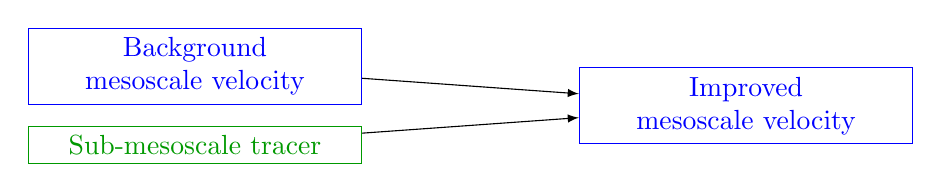
\begin{tikzpicture}
    \node[draw, color=blue, text width=4cm, text centered] (meso) at (0,0) {Background mesoscale velocity};
    \node[draw, color=green!60!black, text width=4cm, text centered](subm) at (0,-1) {Sub-mesoscale tracer};
    \node[draw, color=blue, text width=4cm, text centered] (cor) at (7,-0.5) {Improved mesoscale velocity};
    \draw[->,>=latex] (meso)--(cor);
    \draw[->,>=latex] (subm)--(cor);
  \end{tikzpicture}
  \vspace{0.6cm}
  \begin{block}{Find the correction of this background the most compatible with tracer information}
    \begin{itemize}
     \item The direct measure of the distance between $\vec{\bf{u}}$ and \textbf{Tracer} is not possible
     \item Need to find a go-between variable
     \item Use of Finite-Size Lyapunov Exponents as a proxy (FSLE)
    \end{itemize}
  \end{block}
  %\begin{block}{}
    \small{See Gaultier \& al, 2012 for details}
\end{frame}

\begin{frame}
%\frametitle{What is a FSLE}

\end{frame}
%%%%%%%%%%%%%%%%%%%%%%%%%%%%%%%%%%%%%%%%%%%%%%%%%%%%%%%%%%%%%%%%%%%%%%%%%%%

       \subsection{Consistency of FSLE as a proxy}
%%%%%%%%%%%%%%%%%%%%%%%%%%%%%%%%%%%%%%%%%%%%%%%%%%%%%%%%%%%%%%%%%%%%%%%%%%%%%
\begin{frame}
%\frametitle{Proxy FSLE consistent}
%The FSLE is our proxy
%What is the FSLE
  \begin{columns}
    \begin{column}{0.5\textwidth}
      \begin{figure}%[!htbp]
        \includegraphics[width=6cm]{pict/fsle_24_stat_reg_20814_s_atl.png}\\
        \legende{FSLE, South Atlantic region, \\December 27, 2006}
      \end{figure}
    \end{column}
    \begin{column}{0.5\textwidth}
      \begin{figure}
        \includegraphics[width=6cm]{pict/A2006360165000_L2_LAC_SST.png}\\
        \legende{Tracer (SST), South Atlantic region, \\December 27, 2006}
      \end{figure}
    \end{column}
  \end{columns}
  \vspace{0.5cm}
  \begin{block}{}
  Lyapunov measures stirring in a fluid \\
  $\rightarrow$ Link between sub-mesoscale dynamics and biologic stirring. \\
  (Lehahn \& al, 2008, d'Ovidio \& al, 2004)
  \end{block}
  Maximum lines of Lyapunov exponents and frontal tracer structures present similar patterns (d'Ovidio \& al (2004)).

\end{frame}
%%%%%%%%%%%%%%%%%%%%%%%%%%%%%%%%%%%%%%%%%%%%%%%%%%%%%%%%%%%%%%%%%%%%%%%%

\section{Method of Inversion}
%%%%%%%%%%%%%%%%%%%%%%%%%%%%%%%%%%%%%%%%%%%%%%%%%%%%%%%%%%%%%%%%%%%%%%%%%
%\begin{frame}
%  \frametitle{Methodoligical aspects}
%  \tableofcontents[hideotherpart,currentsection]
%\end{frame}
%%%%%%%%%%%%%%%%%%%%%%%%%%%%%%%%%%%%%%%%%%%%%%%%%%%%%%%%%%%%%%%%%%%%%%%%

	\subsection{Overview of the method}
%%%%%%%%%%%%%%%%%%%%%%%%%%%%%%%%%%%%%%%%%%%%%%%%%%%%%%%%%%%%%%%%%%%%%%%%
\begin{frame}
%\frametitle{Inversion Method}
 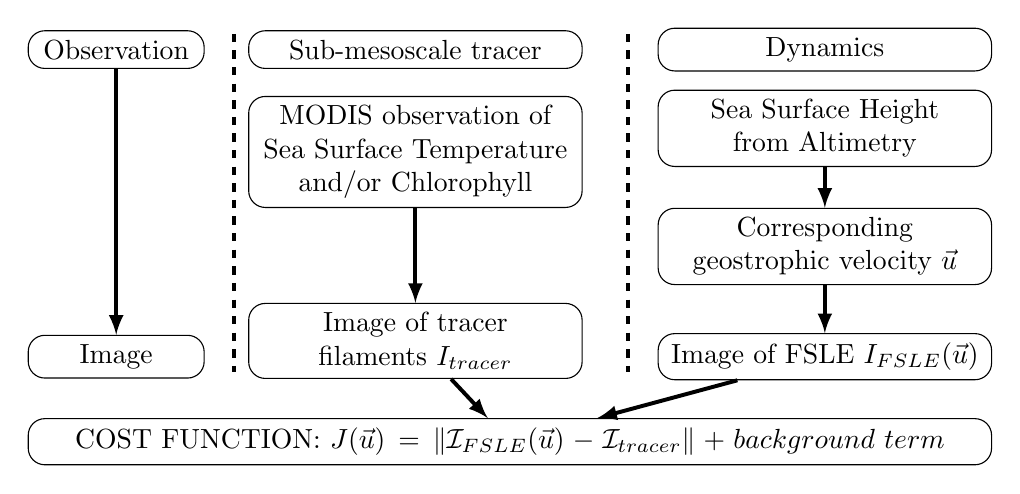
\begin{tikzpicture}
    \tikzset{pname/.style={draw,rectangle,rounded corners=6pt},text centered,color=black}
    \tikzstyle{fleche}=[->,>=latex,line width=0.5mm]
    \node[pname,text width=2cm] (OBS) at (4,8.98) {Observation};
    \node[pname,text width=2cm] (IM) at (4,5.08) {Image};
    \draw[fleche] (OBS)--(IM);
    \draw[dashed,line width=0.5mm] (5.5,9.18)--(5.5,4.88);

    \node[pname,text width=4cm] (TRA) at (7.8,8.98) {Sub-mesoscale tracer};
    \node[pname,text width=4cm] (DYN) at (13,8.98) {Dynamics};
    \draw[dashed,line width=0.5mm] (10.5,9.18)--(10.5,4.88);
    \node[pname,text width=4cm] (OBSTRA) at (7.8,7.68) {MODIS observation of Sea Surface Temperature and/or Chlorophyll};
    \node[pname,text width=4cm] (OBSSSH) at (13,7.98) {Sea Surface Height from Altimetry};
    \node[pname,text width=4cm] (OBSUV) at (13,6.48) {Corresponding geostrophic velocity $\vec{u}$};
    \draw[fleche] (OBSSSH)--(OBSUV);

    \node[pname, text width=4cm] (IMTRA) at (7.8,5.28) {Image of tracer filaments $I_{tracer}$};
    \node[pname,text width=4cm] (IMDYN) at (13,5.08) {Image of FSLE $I_{FSLE}(\vec{u})$};
    \draw[fleche] (OBSTRA)--(IMTRA);
    \draw[fleche] (OBSUV)--(IMDYN);

   \node[pname, text width=12cm] (J) at (9,4.00) {COST FUNCTION: $J(\vec{u})=\|\mathcal{I}_{FSLE}(\vec{u}) -\mathcal{I}_{tracer}\| + background\ term$};
   \draw[fleche] (IMTRA)--(J);
   \draw[fleche] (IMDYN)--(J);
  \end{tikzpicture} \\
\end{frame}

	\subsection{Cost function}
%%%%%%%%%%%%%%%%%%%%%%%%%%%%%%%%%%%%%%%%%%%%%%%%%%%%%%%%%%%%%%%%%%%%%%%%%%%%%%%%%%%%%%%%%%%%%%%%%%%%%%
\begin{frame}
%\frametitle{Inversion Method}
  \begin{block}{}
    $\bullet$ Cost function:
    $$J(u)=\|\lambda(u)- \lambda_{obs}\| + background\ term $$
    The cost function is strongly non linear, with many local minima.\\
%\alt<2>{\centering\includegraphics[width=0.5\linewidth]{J2_med19904.png}\includegraphics[width=0.5\linewidth]{Jiter_record6_HR.png}\\}
%  {
  \end{block}
  \vspace{0.6cm}
  \begin{block}{}
    $\bullet$ Explore sub-space of errors to find the velocity that minimizes the cost function. \\
    Velocity panel using Principal Component Analysis (EOF analysis) with all velocity fields available:
    $$\textbf{u}_k = \bar{\textbf{u}} + \sum_{i=0}^n{\underbrace{a_k^i}_{Eigenvalue}\underbrace{\textbf{u}^i}_{EOF_{}}}$$
    The number of degrees of freedom is reduced, using only 100 or less EOFs. \\
  \end{block}
  \vspace{0.2cm}

%DA Parameters )subspace of error, decreasing algorithm, Gibbs algorithm
\end{frame}
%%%%%%%%%%%%%%%%%%%%%%%%%%%%%%%%%%%%%%%%%%%%%%%%%%%%%%%%%%%%%%%%%%%%%%%%

\part{Results of the Inversion}

%-------------------------------------------%
%%%%%%%%%%%%%%%%%%%%%%%%%%%%%%%%%%%%%%%%%%%%%%%%%%%%%%%%%%%%%%%%%%%%%%%%%
\begin{frame}
  \frametitle{\insertromanpartnumber \hspace{1em} \insertpart}
  \tableofcontents[hideotherpart]
\end{frame}
%%%%%%%%%%%%%%%%%%%%%%%%%%%%%%%%%%%%%%%%%%%%%%%%%%%%%%%%%%%%%%%%%%%%%%%

\section[Real data]{Feasability study using real observations}
%%%%%%%%%%%%%%%%%%%%%%%%%%%%%%%%%%%%%%%%%%%%%%%%%%%%%%%%%%%%%%%%%%%%%%%%%
%\begin{frame}
%  \frametitle{Methodoligical aspects}
%  \tableofcontents[hideotherpart,currentsection]
%\end{frame}
%%%%%%%%%%%%%%%%%%%%%%%%%%%%%%%%%%%%%%%%%%%%%%%%%%%%%%%%%%%%%%%%%%%%%%%%


	\subsection{Test case in the South Atlantic ocean}
%%%%%%%%%%%%%%%%%%%%%%%%%%%%%%%%%%%%%%%%%%%%%%%%%%%%%%%%%%%%%%%%%%%%%%%%
\begin{frame}
%  \frametitle{Test case : small area in the South Atlantic ocean}
  \begin{tikzpicture}
    \node[anchor=west,inner sep=0] (pict) at (-6,0){\includegraphics[width=4.5cm]{./pict/satl/pict_sst_A20060172006024_L3m_8D_SST_9_atl.jpg}};
    \node[anchor= west,inner sep=0] (picts) at (0,0){\includegraphics[width=2.5cm]{./pict/satl/A2006019163000_L2_LAC_SST.png}};
    \draw[dashed,line width=0.25mm] (-3.75,-0.8)--(0.25,1.15);
    \draw[dashed,line width=0.25mm] (-3.75,-1.1)--(0.25,-1.05);
  \end{tikzpicture}

%  \begin{figure}
 %   \includegraphics[width=0.5\linewidth]{pict/satl/pict_sst_A20060172006024.L3m_8D_SST_9_atl.jpg}
 %    \includegraphics[width=0.5\linewidth]{pict/satl/A2006019163000_L2_LAC_sst.png}
%  \end{figure}
  \begin{itemize}
    \item \textbf{Time Range}: from 1998 to June 2009, 595 velocity maps
    \item \textbf{Velocity field}: AVISO, Altimetric data
    \item \textbf{Resolution}: $1/3^o$, grid points : 13*17
    \item \textbf{FSLE Resolution}: $1/50^o$, grid points : 99*130
  \end{itemize}
%  \vsapce{1cm}
  \begin{itemize}
    \item \textbf{Tracer field}: SST or Chlorophyll data (MODIS sensor, L2 product)
    %resolution needed to detect filament $1/100^o$, to match fsle $1/50^o$
  \end{itemize}

\end{frame}
%%%%%%%%%%%%%%%%%%%%%%%%%%%%%%%%%%%%%%%%%%%%%%%%%%%%%%%%%%%%%%%%%%%%%%%%

	\subsection[Cost function]{Study of the cost function}
%%%%%%%%%%%%%%%%%%%%%%%%%%%%%%%%%%%%%%%%%%%%%%%%%%%%%%%%%%%%%%%%%%%%%%%%
\begin{frame}
%Evolution of the cost function for synthetic inversion, real data inversion
 \centering
%\alt<2>{\frametitle{Study of the cost function: Full inversion}}
 %      {\frametitle{Study of the cost function: Inversion of FSLE}}

  \begin{center}
  \alt<2>{STEP 2}{STEP1}
  \end{center}
  \begin{columns}
    \begin{column}{0.49\textwidth}
    \begin{center}
     Explore the cost function around the solution \\
  \alt<2>{\includegraphics[width=0.78\linewidth]{pict/satl/J1D_tra0s_atl3_1_10.png}}{}
     \end{center}
    \end{column}
    \begin{column}{0.49\textwidth}
     \begin{center}
     Cost function as a function of the number of iterations \\
     \alt<2>{\includegraphics[width=0.78\linewidth]{pict/satl/Jiter_20471_s_atl2.png}}{}
    \end{center}
     \end{column}
     \end{columns}
 \begin{block}{}
  \alt<2>{Use of Simulated Annealing to decrease the cost function.\\
          Use of Gibbs' sampler to get a sample of the likely solutions.}
  {Cost Function : $J(u)=\|\mathcal{I}_{FSLE}(\vec{u})- \mathcal{I}_{tracer}\| + background\ term $}
  \end{block}
\end{frame}
%%%%%%%%%%%%%%%%%%%%%%%%%%%%%%%%%%%%%%%%%%%%%%%%%%%%%%%%%%%%%%%%%%%%%%%%  

	\subsection{Corrected velocity field}
%%%%%%%%%%%%%%%%%%%%%%%%%%%%%%%%%%%%%%%%%%%%%%%%%%%%%%%%%%%%%%%%%%%%%%%%
\begin{frame}
%Corrections on ssh and u,v
\end{frame}

\begin{frame}
%Lagrangian trajectories
\end{frame}
%%%%%%%%%%%%%%%%%%%%%%%%%%%%%%%%%%%%%%%%%%%%%%%%%%%%%%%%%%%%%%%%%%%%%%%%

\section[Process model data]{Validation of the method on a process model}
%------------------------------------------------------------------------%
%%%%%%%%%%%%%%%%%%%%%%%%%%%%%%%%%%%%%%%%%%%%%%%%%%%%%%%%%%%%%%%%%%%%%%%%%
%\begin{frame}
%  \frametitle{Methodoligical aspects}
%  \tableofcontents[hideotherpart,currentsection]
%\end{frame}
%%%%%%%%%%%%%%%%%%%%%%%%%%%%%%%%%%%%%%%%%%%%%%%%%%%%%%%%%%%%%%%%%%%%%%%%


	\subsection{Model data}
%%%%%%%%%%%%%%%%%%%%%%%%%%%%%%%%%%%%%%%%%%%%%%%%%%%%%%%%%%%%%%%%%%%%%%%%
\begin{frame}
%Physicobiogeochemical Model
\end{frame}
%%%%%%%%%%%%%%%%%%%%%%%%%%%%%%%%%%%%%%%%%%%%%%%%%%%%%%%%%%%%%%%%%%%%%%%%

	\subsection{Inversion of a tracer image from the model}
%%%%%%%%%%%%%%%%%%%%%%%%%%%%%%%%%%%%%%%%%%%%%%%%%%%%%%%%%%%%%%%%%%%%%%%%
\begin{frame}
%Inversion with SST alone, Chl alone, SST and Chl, bidouille SST+Chl 
\end{frame} 
%%%%%%%%%%%%%%%%%%%%%%%%%%%%%%%%%%%%%%%%%%%%%%%%%%%%%%%%%%%%%%%%%%%%%%

	\subsection{Part of the information extracted from the imeage}
%%%%%%%%%%%%%%%%%%%%%%%%%%%%%%%%%%%%%%%%%%%%%%%%%%%%%%%%%%%%%%%%%%%%%%%%
\begin{frame}
%Add information using SST and Chl or other tracer? bidouille SST+Chl 
\end{frame} 
%%%%%%%%%%%%%%%%%%%%%%%%%%%%%%%%%%%%%%%%%%%%%%%%%%%%%%%%%%%%%%%%%%%%%%%%


\section[Realistic Model data]{Limits of inversion using a realistic model}
%-------------------------------------------------------------------------%
%%%%%%%%%%%%%%%%%%%%%%%%%%%%%%%%%%%%%%%%%%%%%%%%%%%%%%%%%%%%%%%%%%%%%%%%%
%\begin{frame}
%  \frametitle{Methodoligical aspects}
%  \tableofcontents[hideotherpart,currentsection]
%\end{frame}
%%%%%%%%%%%%%%%%%%%%%%%%%%%%%%%%%%%%%%%%%%%%%%%%%%%%%%%%%%%%%%%%%%%%%%%%


	\subsection{Model data}
%%%%%%%%%%%%%%%%%%%%%%%%%%%%%%%%%%%%%%%%%%%%%%%%%%%%%%%%%%%%%%%%%%%%%%%%
\begin{frame}
%Salomon model
\end{frame}
%%%%%%%%%%%%%%%%%%%%%%%%%%%%%%%%%%%%%%%%%%%%%%%%%%%%%%%%%%%%%%%%%%%%%%%%

	\subsection{Similarities between FSLE and tracer}
%%%%%%%%%%%%%%%%%%%%%%%%%%%%%%%%%%%%%%%%%%%%%%%%%%%%%%%%%%%%%%%%%%%%%%%%
\begin{frame}
%Annual cycle
\end{frame}
%%%%%%%%%%%%%%%%%%%%%%%%%%%%%%%%%%%%%%%%%%%%%%%%%%%%%%%%%%%%%%%%%%%%%%%%

	\subsection{Inversion of a tracer image}
%%%%%%%%%%%%%%%%%%%%%%%%%%%%%%%%%%%%%%%%%%%%%%%%%%%%%%%%%%%%%%%%%%%%%%%%
\begin{frame}
%Feasability of the inversion 
\end{frame}
%%%%%%%%%%%%%%%%%%%%%%%%%%%%%%%%%%%%%%%%%%%%%%%%%%%%%%%%%%%%%%%%%%%%%%%%

\part{Conclusion}
\section{Prospects and Conclusions}
%------------------------------------------------%

	\subsection{Prospects}
%%%%%%%%%%%%%%%%%%%%%%%%%%%%%%%%%%%%%%%%%%%%%%%%%%%%%%%%%%%%%%%%%%%%%%%%%
\begin{frame}
%Full DA
%SWOT Prospects
\end{frame}
%%%%%%%%%%%%%%%%%%%%%%%%%%%%%%%%%%%%%%%%%%%%%%%%%%%%%%%%%%%%%%%%%%%%%%%%%

	\subsection{Conclusions}
%%%%%%%%%%%%%%%%%%%%%%%%%%%%%%%%%%%%%%%%%%%%%%%%%%%%%%%%%%%%%%%%%%%%%%%%%
\begin{frame}
%Conclusions
\end{frame}
%%%%%%%%%%%%%%%%%%%%%%%%%%%%%%%%%%%%%%%%%%%%%%%%%%%%%%%%%%%%%%%%%%%%%%%%%

%%%%%%%%%%%%%%%%%%%%%%%%%%%%%%%%%%%%%%%%%%%%%%%%%%%%%%%%%%%%%%%%%%%%%%%%%
\begin{frame}
\begin{center}
Thank you for your attention 
\end{center}
\end{frame}
%%%%%%%%%%%%%%%%%%%%%%%%%%%%%%%%%%%%%%%%%%%%%%%%%%%%%%%%%%%%%%%%%%%%%%%%%
\end{document}
